\documentclass[11pt,letterpaper]{article}
\usepackage[utf8]{inputenc}
\usepackage[top=1in,bottom=1in,left=1in,right=1in]{geometry}
\usepackage{amsmath}
\usepackage{amsfonts}
\usepackage{amssymb}
\usepackage{amsthm}
\usepackage{bm}
\usepackage{braket}
\usepackage{cancel}
\usepackage{enumitem}
\usepackage{float}
\usepackage[T1]{fontenc}
\usepackage{forloop}
\usepackage{graphicx}
\usepackage{hyperref}
\usepackage{lmodern}
\usepackage{mathabx}
\usepackage{parskip}
\usepackage{subcaption}
\usepackage{tensor}
\usepackage{titlesec}
\usepackage{titling}
\usepackage{listings}

\lstset{basicstyle=\footnotesize\ttfamily}

\setenumerate{leftmargin=*}


% \titlelabel{(\thetitle)\quad}
\titleformat*{\section}{\large\bfseries}
\titleformat*{\subsection}{\normalsize\bfseries}
\setlength{\droptitle}{-5em}


\DeclareMathOperator*{\argmin}{arg\,min}
\DeclareMathOperator*{\argmax}{arg\,max}

\DeclareMathOperator{\tr}{tr}

\let\Re\relax
\DeclareMathOperator{\Re}{Re}
\let\Im\relax
\DeclareMathOperator{\Im}{Im}

\DeclareMathOperator{\sgn}{sgn}

\newcommand{\R}{\mathbb{R}}


\theoremstyle{definition}
\newtheorem{defn}{Definition}[section]

\theoremstyle{plain}
\newtheorem{thm}{Theorem}[section]



\newcommand{\bhat}[1]{\hat{\bm{#1}}}
\newcommand{\prop}{\mathrel{\propto}}


\renewcommand{\thesubsection}{\normalsize \alph{subsection}}
\renewcommand{\d}{\mathrm{d}}
\renewcommand{\vec}[1]{\bm{#1}}
\newcommand{\del}{\vec{\nabla}}
\newcommand{\e}{\epsilon}
\newcommand{\tpd}[3]{\left( \frac{\partial #1}{\partial #2} \right)_{#3}}
\newcommand{\pd}[2]{\frac{\partial #1}{\partial #2}}
\newcommand{\spd}[2]{\frac{\partial^2 #1}{\partial {#2}^2}}
\def\dbar{{\mathchar'26\mkern-12mu d}}

\allowdisplaybreaks

\author{Sam Kowash}
\numberwithin{equation}{section}
\numberwithin{figure}{section}
\title{CSE 546 HW \#4}

\begin{document}
\maketitle

{\bf Acknowledgments:} I collaborated with Tyler Blanton and Michael Ross.

\section{Expectation maximization}
\begin{enumerate}
	\item Suppose that we have a set of feature vectors $x_1, \ldots, x_n \in \R^d$, where each vector represents a song, and a sample set $\mathcal{S} \subset \{1,\ldots,n\}$ of listen counts $Y_i \in \mathbb{Z}^+$ for a given user. We assume $Y_i \sim \mathrm{Poisson}(\lambda_i)$, where $\lambda_i \equiv \mathbb{E}[Y_i \mid x_i]$ and we assume a model $\lambda_i = \exp(w^T x_i)$ for some $w \in \R^d$.

	\begin{enumerate}
		\item The MLE estimator for this model is
		%
		\begin{align*}
			\hat{w} &= \argmax_w \prod_{i \in \mathcal{S}} \frac{\exp(y_i x_i^T w)}{y_i!} \exp\left[-e^{w^T x_i}\right].
		\end{align*}
		%
		There is no closed-form solution for $\hat{w}$, but observe that
		%
		\begin{align*}
			\argmax_w \prod_{i \in \mathcal{S}} \frac{\exp(y_i x_i^T w)}{y_i!} \exp\left[-e^{w^T x_i}\right] &= \argmax_w \exp\left\{-\sum_{i\in\mathcal{S}}\left[e^{x_i^T w} - y_i x_i^T w\right]\right\},
		\end{align*}
		%
		and the exponential is maximized when the negative of its exponent is minimized, so
		\begin{align*}
			\hat{w} &= \argmin_w \sum_{i\in\mathcal{S}}\left[e^{x_i^T w} - y_i x_i^T w\right]. \
		\end{align*}
		%
		Note that the Hessian of each term in the sum is
		%
		\begin{align*}
			\nabla^2_w \hat{w}_i &= x_i x_i^T,
		\end{align*}
		%
		which we showed in HW 0 is PSD. The Hessian of the whole objective is then a sum of PSD matrices which is itself PSD, and since a function with PSD Hessian is convex, finding $\hat{w}$ is a convex optimization problem. We can solve for it with a number of methods, including, for example, SGD and Newton's method.



		\item Suppose we now determine that each song $x_i$ belongs to one of $k$ unknown moods, each of which should have its own weight vector, and want to estimate these clusters from the observed data.



	\end{enumerate}
\end{enumerate}



\section{Regression with side information}
\begin{enumerate}
	\setcounter{enumi}{1}
	\item We implement kernel regression with the rbf kernel via \texttt{cvxpy} on $n=50$ points $y_i$ drawn from the graph of
	%
	\begin{align*}
		f(x) &= 10\sum_{k=1}^4 \bm{1}\{x\geq \frac{k}{5}\}
	\end{align*}
	%
	on $[0,1]$ with Gaussian noise $\e_i \sim \mathcal{N}(0,1)$ applied to each point $x_i$ and one deliberate outlier $y_{25} = 0$.

	Throughout, we use the rbf kernel,
	%
	\begin{align*}
		k(x_1,x_2) = \exp(-\gamma|x_1-x_2|^2),
	\end{align*}
	%
	where $\gamma>0$ is a hyperparameter, and the estimator
	%
	\begin{align}
		\hat{f}(x) &= \sum_{i=1}^n \hat{\alpha}_i k(x_i, x),
	\end{align}
	%
	where $\alpha$ is the weight vector to optimize.

	\begin{enumerate}
		\item We first optimize the usual regularized least-squares objective
		%
		\begin{align*}
			J(\alpha) &= \sum_{i=1}^n \ell_\mathrm{LS}\left(y_i - \sum_{j=1}^n K_{ij} \alpha_j\right) + \lambda \alpha^T K \alpha,
		\end{align*}
		%
		where $K_{ij} = k(x_i,x_j)$. We used LOOCV over the data points to evaluate randomly-selected hyperparameters $(\lambda, \gamma)$, producing the loss contours in Fig.~\ref{fig:2a_loocv}.


		\begin{figure}[H]
			\centering
			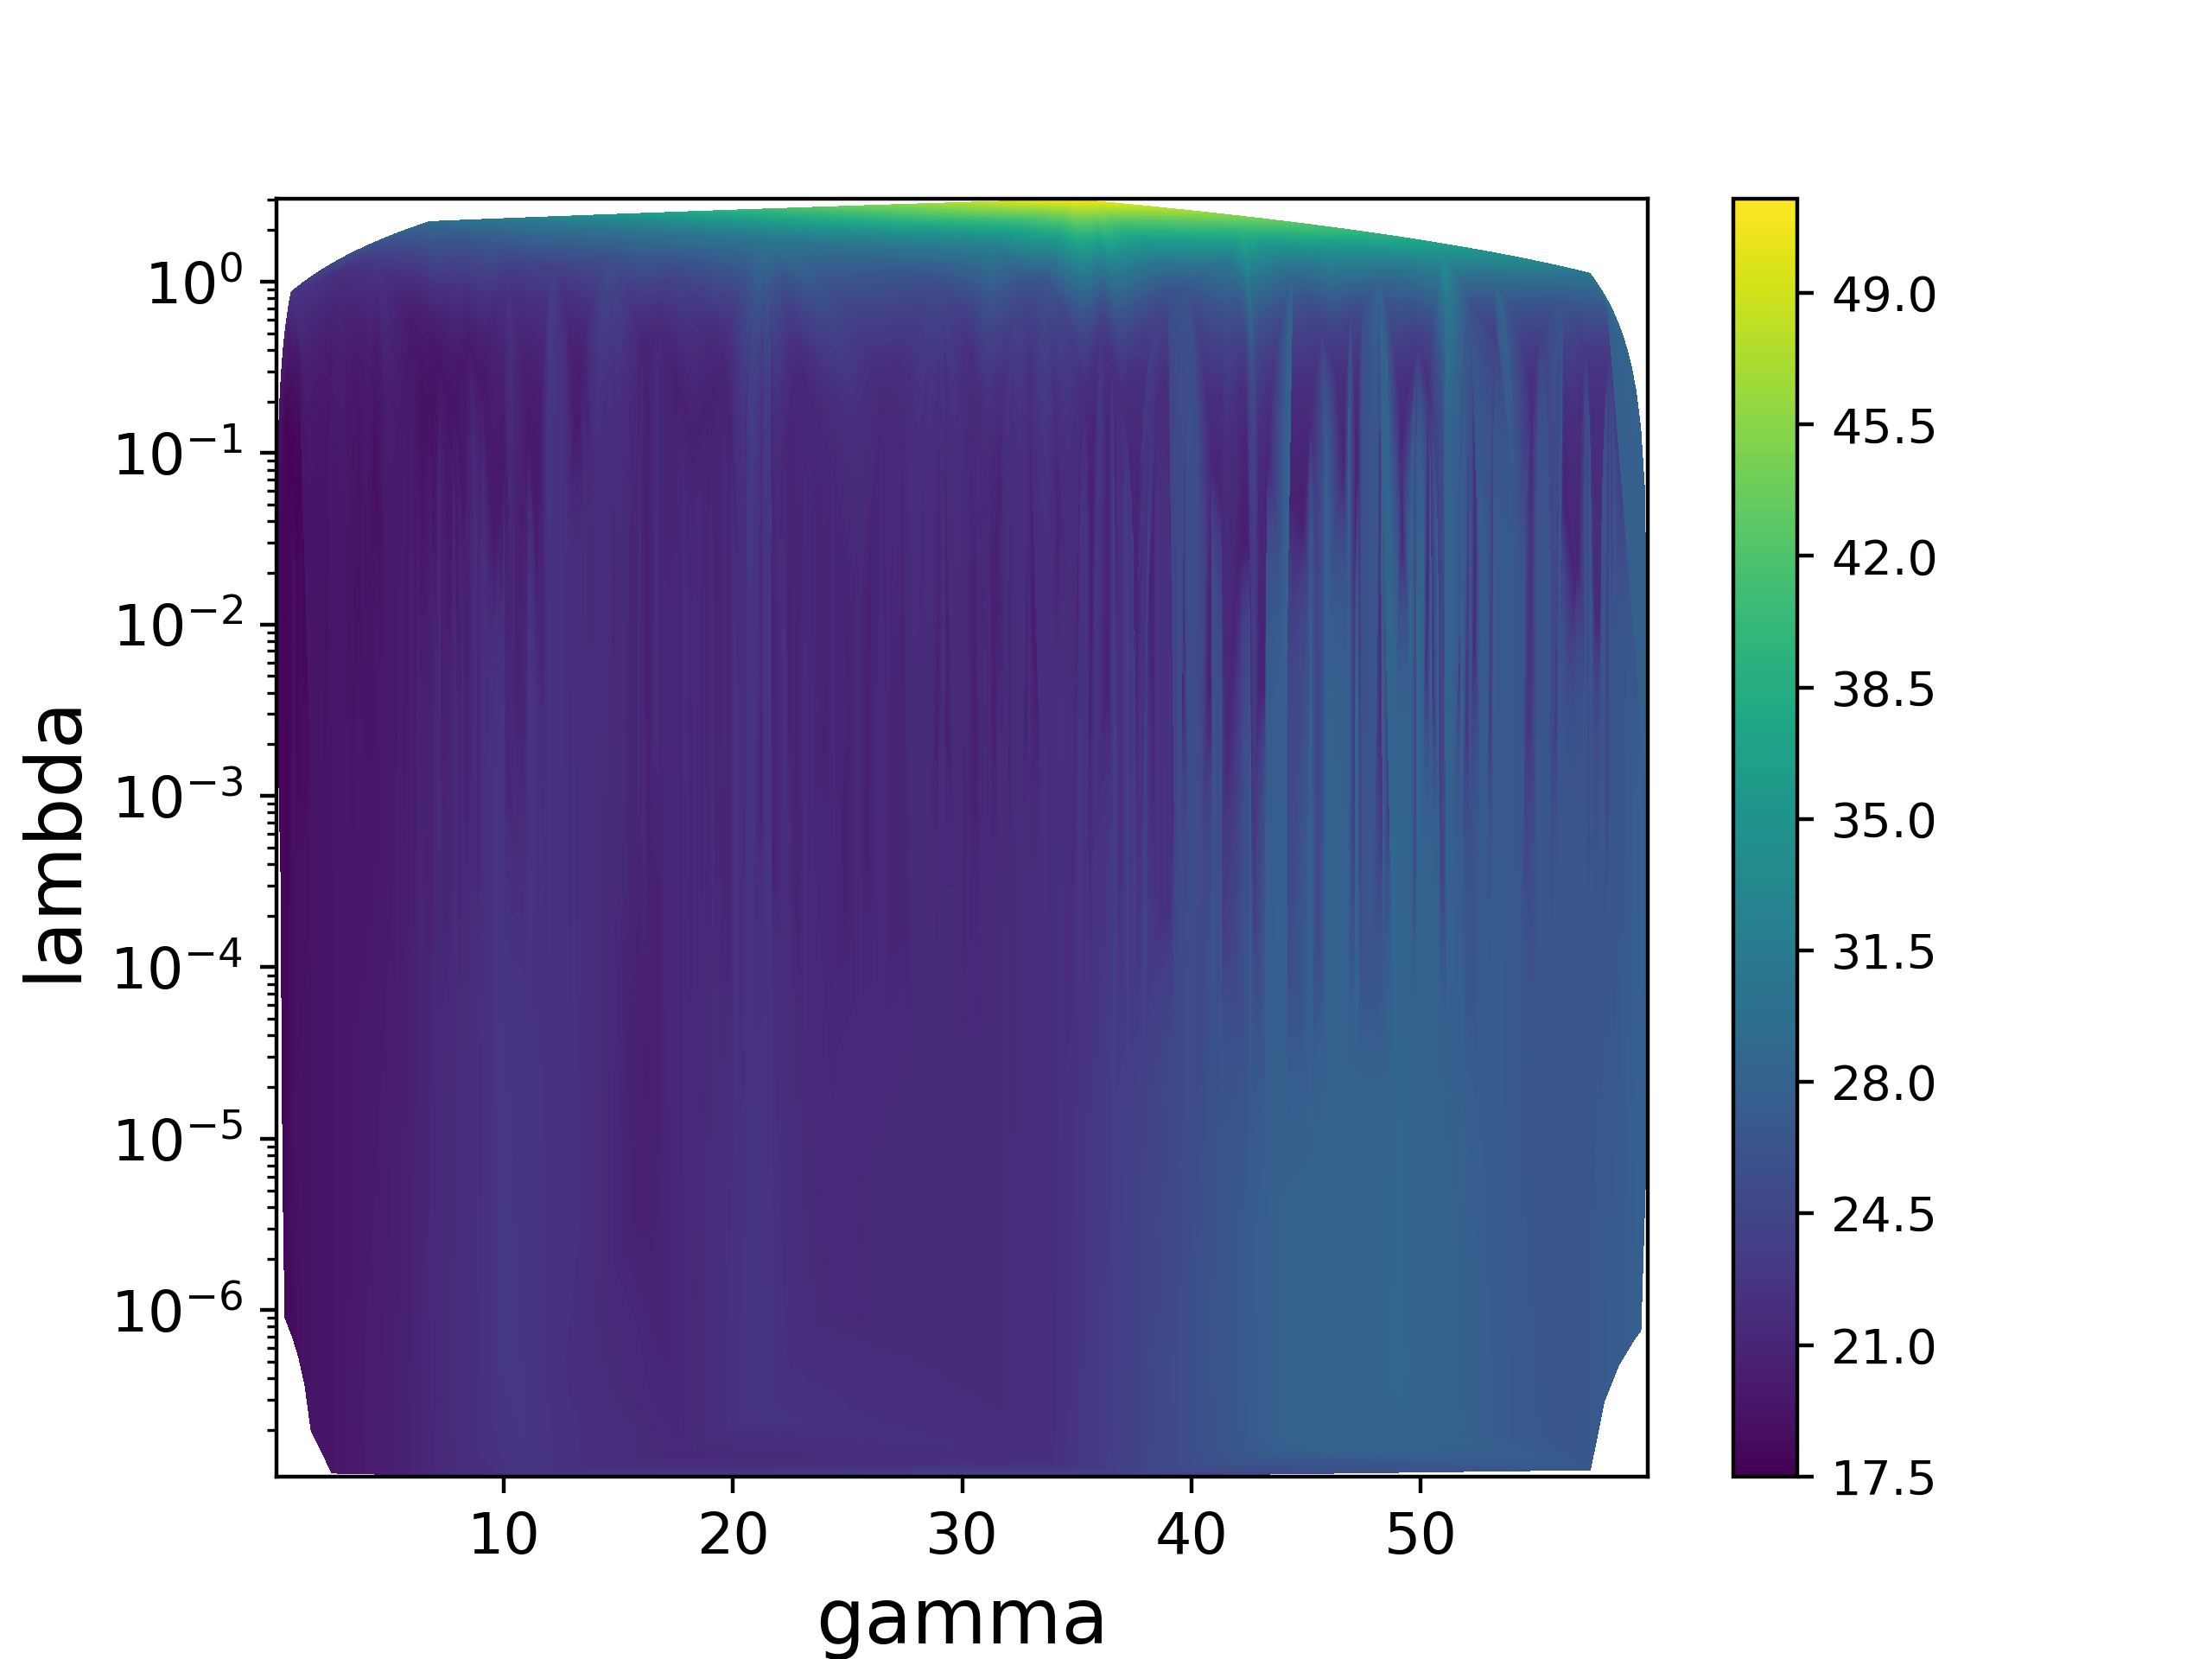
\includegraphics[width=.6\textwidth]{figures/2a_loocv.png}
			\caption{LOOCV loss contours for random values of $(\lambda, \gamma)$}
			\label{fig:2a_loocv}
		\end{figure}

		From this, we estimated $\gamma=16$ and $\lambda = 1.5\times 10^{-5}$ as reasonable hyperparameters (although the loss surface appears very flat in large regions of the parameter space).


		\item We next considered optimizing the Huber loss summed over the data set. A similar LOOCV procedure produced figure
		%
		\begin{figure}[H]
			\centering
			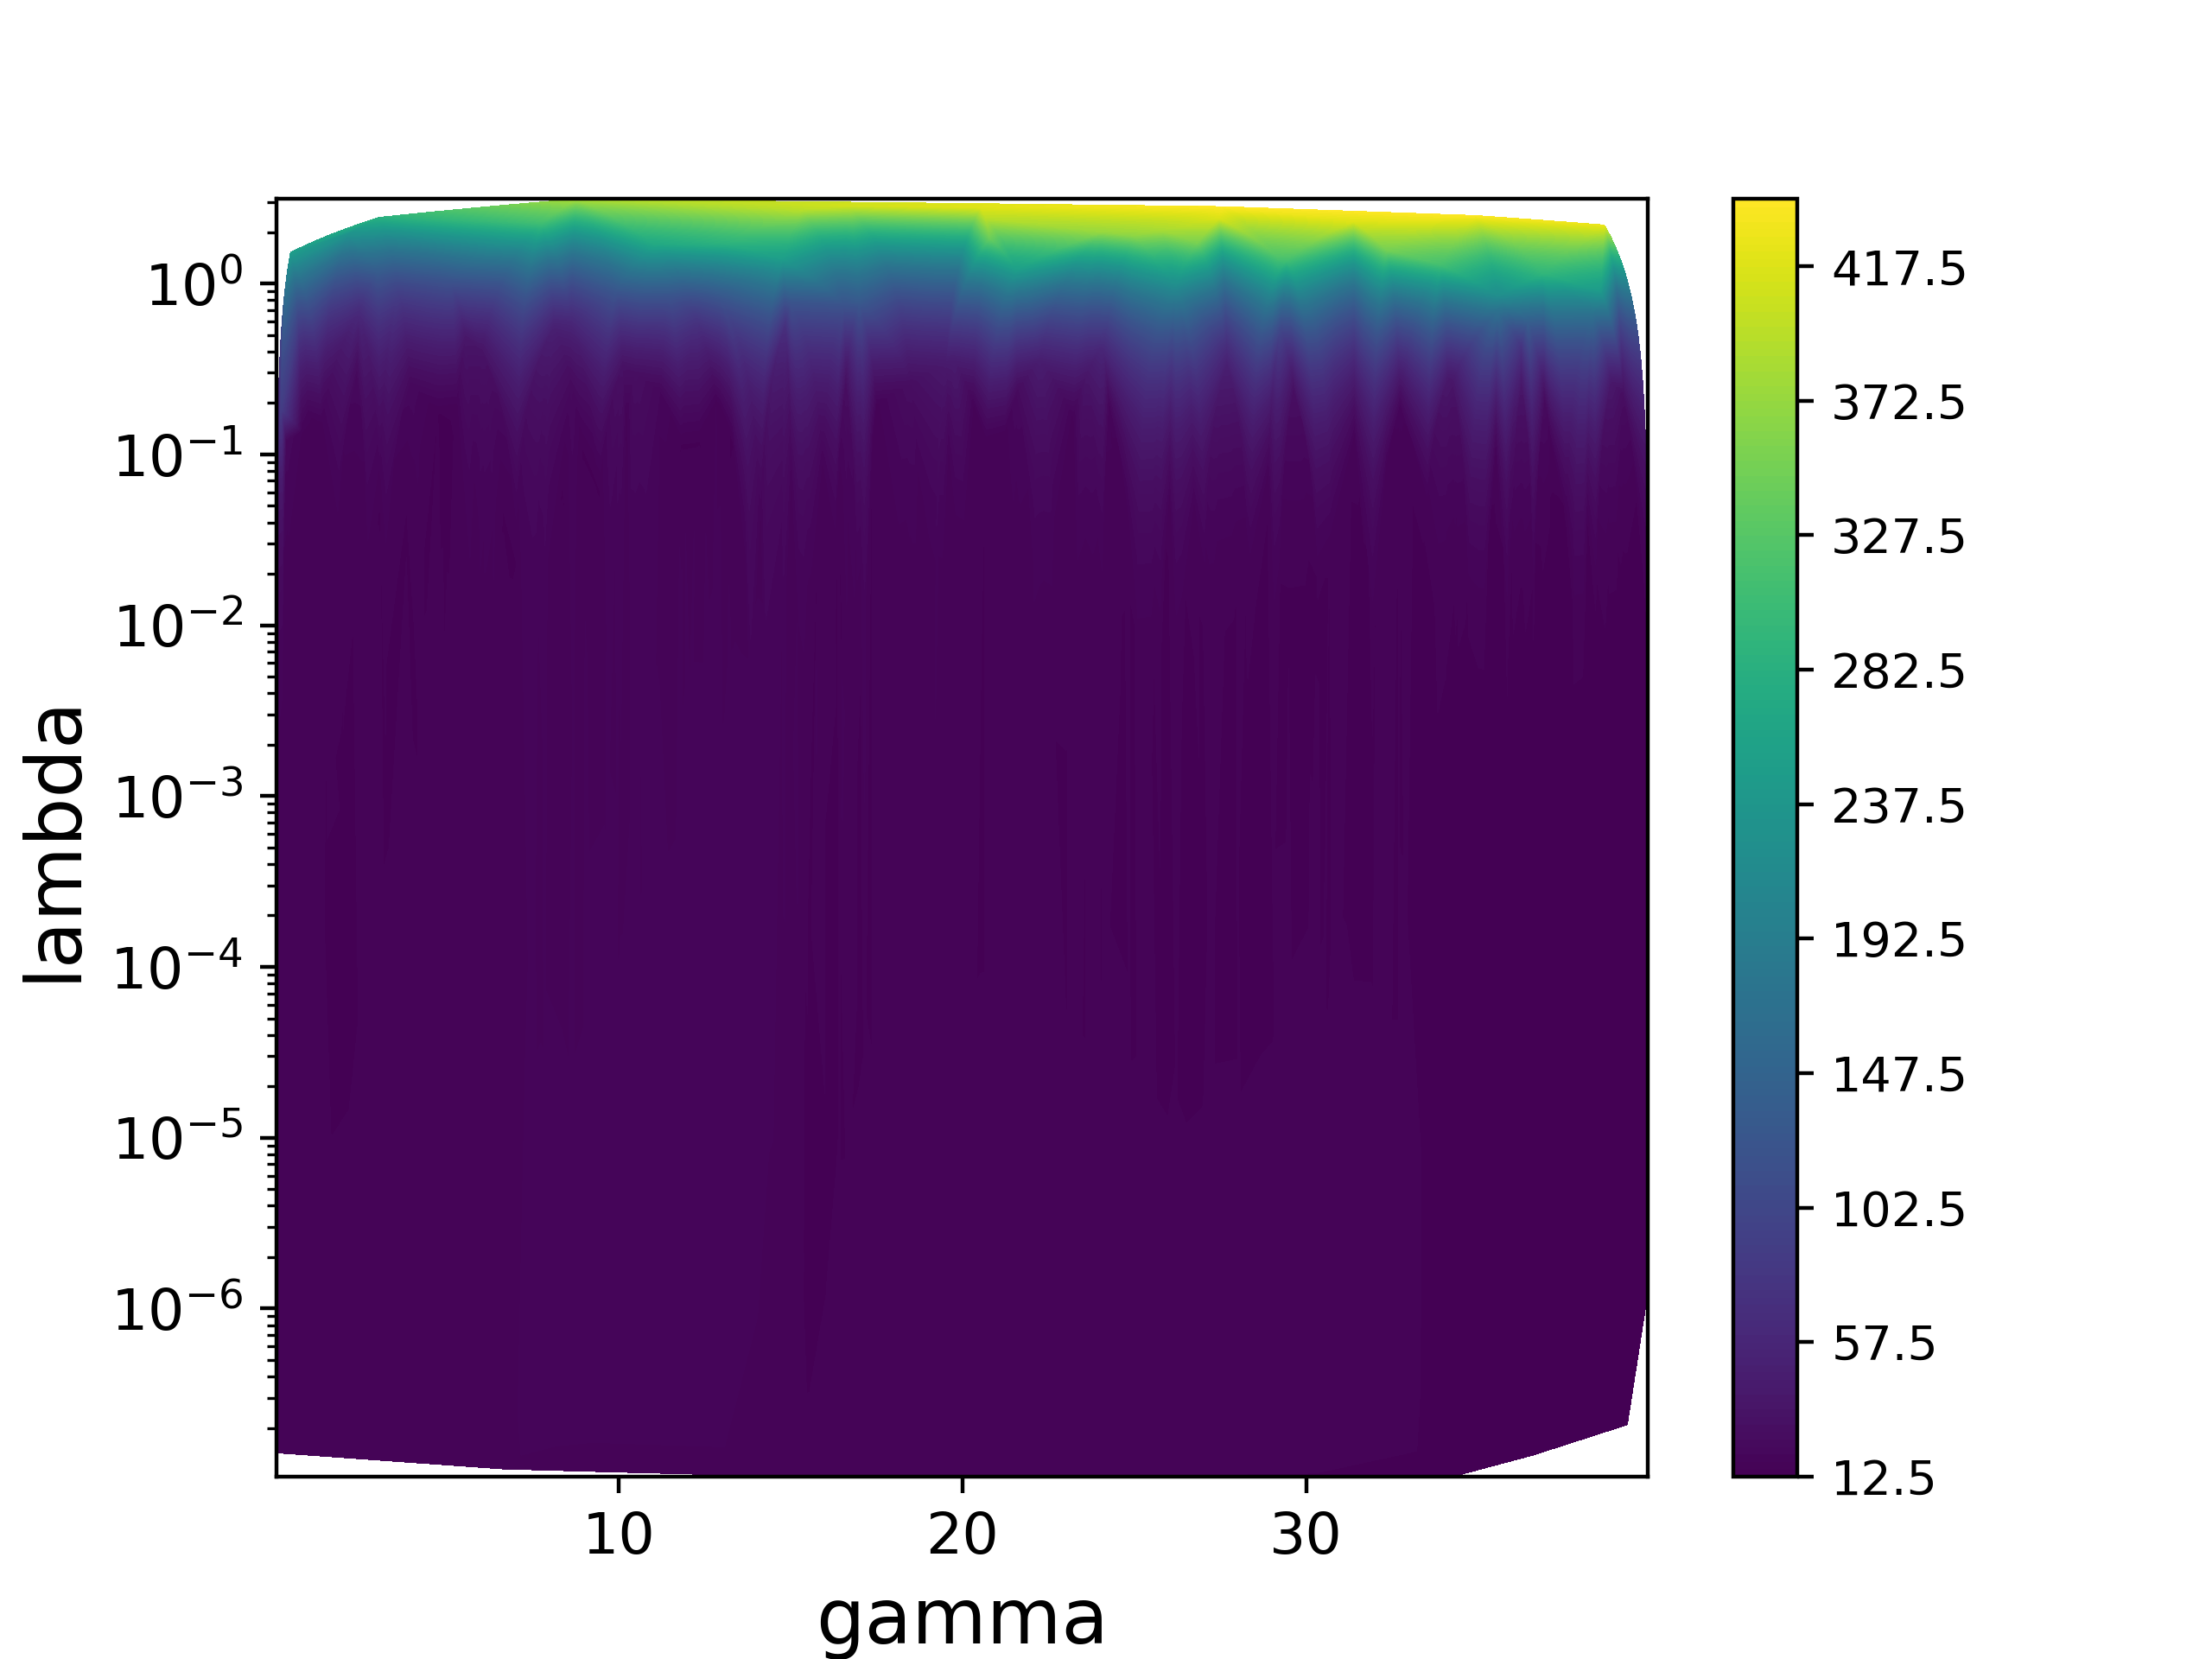
\includegraphics[width=.6\textwidth]{figures/2b_loocv.png}
			\caption{LOOCV loss contours for random values of $(\lambda,\gamma)$}
			\label{fig:2b_loocv}
		\end{figure}
		%
		This is, if anything, harder to interpret visually, but with a well-scaled set of contours (not shown), we determined $\gamma =2$ and $\lambda = 10^{-4}$ as appropriate hyperparameter values.
	\end{enumerate}

\end{enumerate}





\section{Deep learning architectures}
\begin{enumerate}
	\setcounter{enumi}{2}
	\item

	\item
	\begin{figure}[H]
		\centering
		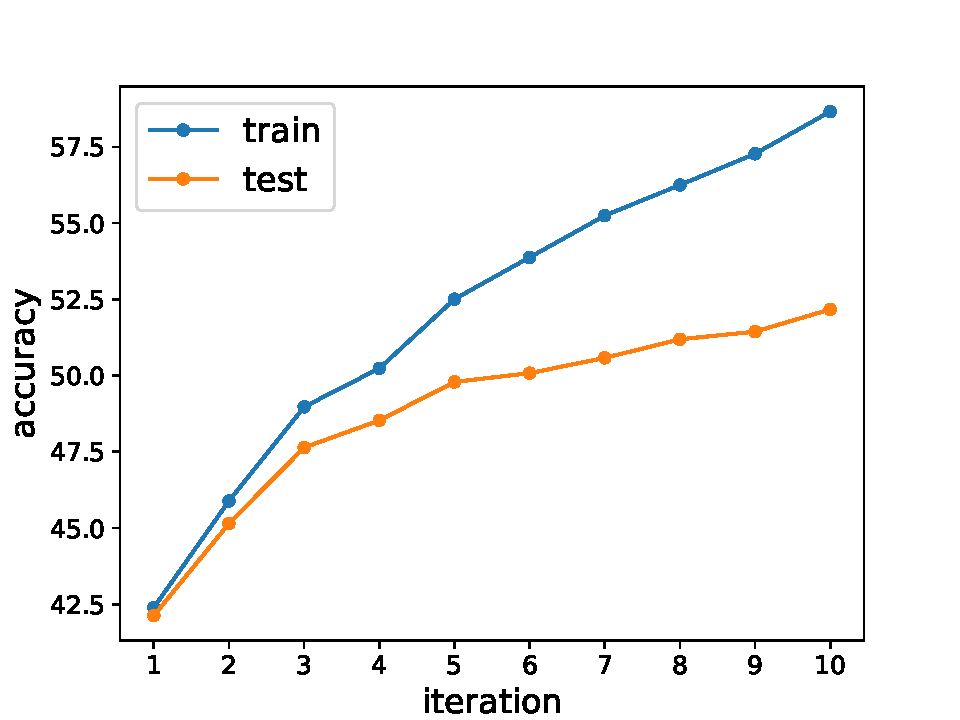
\includegraphics[width=.6\textwidth]{figures/3b_acc.pdf}
		\caption{Accuracy curves for NN with single fully-connected hidden layer; learning rate of $5\times10^{-4}$, momentum of $0.5$, and $M=150$}
	\end{figure}

	\item
	\begin{figure}[H]
		\centering
		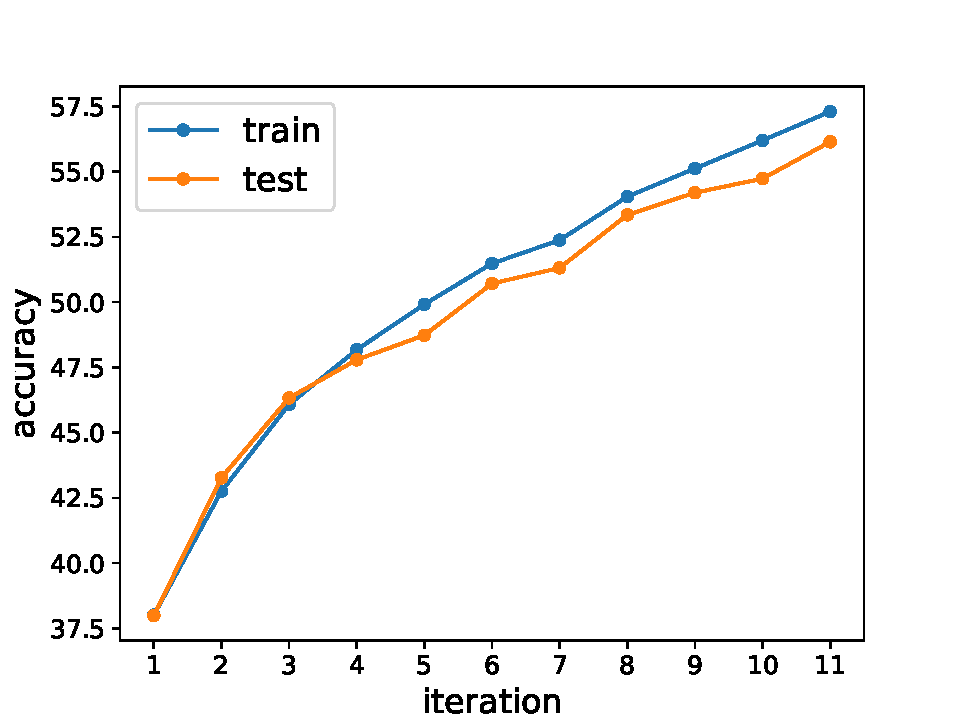
\includegraphics[width=.6\textwidth]{figures/3c_acc.pdf}
		\caption{Accuracy curves for NN with convolution layer and MaxPool; learning rate of $5\times10^{-4}$, momentum of $0.7$, $M=100$, $p=6$, and $N=9$}
	\end{figure}
\end{enumerate}



\clearpage
\lstinputlisting[language=Python]{code/2a.py}
\clearpage
\lstinputlisting[language=Python]{code/2b.py}
\clearpage
\lstinputlisting[language=Python]{code/3a.py}
\clearpage
\lstinputlisting[language=Python]{code/3b.py}
\clearpage
\lstinputlisting[language=Python]{code/3c.py}
\clearpage
\lstinputlisting[language=Python]{code/plotter.py}
\end{document}